\documentclass[class=article, crop=false]{standalone}
\usepackage{my_preamble}
\begin{document}
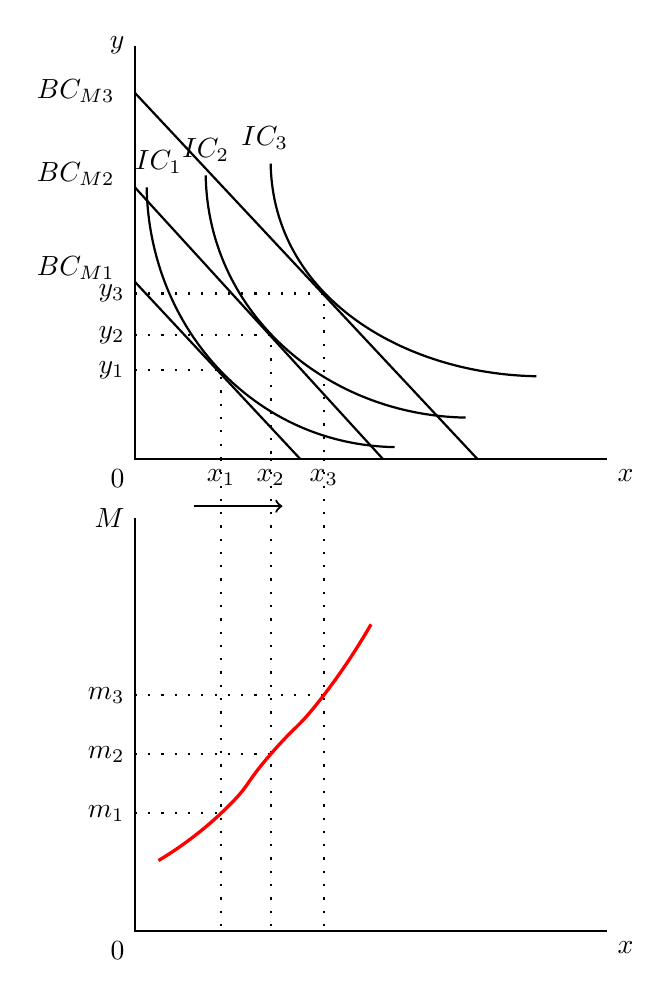
\begin{tikzpicture}[thick,font=\sffamily,scale=1.5]
%axies
 \draw (0,3.5) node[left]{$y$} -- (0,0) node[below left] {$0$} -- (4,0) node[below right]{$x$}; %top graph
 \draw (0,-0.5) node[left]{$M$} -- (0,-4) node[below left] {$0$} -- (4,-4) node[below right]{$x$}; %bottom graph
%top graph
	%equations
		%original
		\draw[] (0,1.5) -- (1.4,0); %BC1
		\draw [thick] (0.1,2.3) to [out=271,in=179] (2.2,0.1); %IC1
		
		%shift1
		\draw[] (0,2.3) -- (2.1,0); %BC2
		\draw [thick] (0.6,2.4) to [out=271,in=179] (2.8,0.35); %IC2
		
		%shift2
		\draw[] (0,3.1) -- (2.9,0); %BC3
		\draw [thick] (1.15,2.5) to [out=271,in=179] (3.4,0.7); %IC3
	
	%dotted lines
	 \draw[loosely dotted] (0,0.75) node[left]{$y_1$} -| node[pos=0.25,below=3mm] {}
	  (0.73,0) node[below]{$x_1$}; %x1 line  
	 \draw[loosely dotted] (0,1.05) node[left]{$y_2$} -| node[pos=0.25,below=3mm] {} (1.15,0) node[below]{$x_2$}; %x2 line 
	 \draw[loosely dotted] (0,1.4) node[left]{$y_3$} -| node[pos=0.25,below=3mm] {} (1.6,0) node[below]{$x_3$}; %x3 and horizontal lines
	  
	\node[below] at (-0.5,1.8) {$BC_{M1}$}; %BC label
	\node[below] at (-0.5,2.6) {$BC_{M2}$}; %BC2 label
	\node[below] at (-0.5,3.3) {$BC_{M3}$}; %BC3 label
	\node[below] at (0.2,2.7) {$IC_{1}$}; %IC1 label
	\node[below] at (0.6,2.8) {$IC_{2}$}; %IC2 label  
	\node[below] at (1.1,2.9) {$IC_{3}$}; %IC3 label
	\draw [->] (0.5,-0.4) -- (1.25,-0.4); %x arrow
	%\draw [->] (-0.5,1.35) -- (-0.5,1.1); %y arrow
%bottom graph-------------------------------
	%x Lines
	\draw[loosely dotted] (0.73,0) -- (0.73,-4); %x1
	\draw[loosely dotted] (1.15,0) -- (1.15,-4); %x2
	\draw[loosely dotted] (1.6,0) -- (1.6,-4); %x3
	
	%m lines
	\draw[loosely dotted] (0,-3) node[left]{$m_1$} -- (0.73,-3); %m1
	\draw[loosely dotted] (0,-2.5) node[left]{$m_2$} -- (1.15,-2.5); %m2
	\draw[loosely dotted] (0,-2) node[left]{$m_3$} -- (1.6,-2); %m3
	
	%Engel curve
	\draw[very thick, red] plot [smooth, tension=1] coordinates{(0.2,-3.4) (0.73,-3) (1.15,-2.5) (1.6,-2) (2,-1.4)}; %part 3
\end{tikzpicture}
\end{document}